% Template:     Informe/Reporte LaTeX
% Documento:    Archivo principal
% Versión:      4.7.3 (05/02/2018)
% Codificación: UTF-8
%
% Autor: Pablo Pizarro R.
%        Facultad de Ciencias Físicas y Matemáticas
%        Universidad de Chile
%        pablo.pizarro@ing.uchile.cl, ppizarror.com
%
% Manual template: [http://latex.ppizarror.com/Template-Informe/]
% Licencia MIT:    [https://opensource.org/licenses/MIT/]

% CREACIÓN DEL DOCUMENTO
\documentclass[letterpaper,11pt]{article} % Articulo tamaño carta, 11pt
\usepackage[utf8]{inputenc} % Codificación UTF-8

% INFORMACIÓN DEL DOCUMENTO
\def\titulodelinforme {Tarea 3}
\def\temaatratar {Prototipo de Implementación}

\def\autordeldocumento {Grupo 4: Soft, where?}
\def\nombredelcurso {Ingeniería de Software I}
\def\codigodelcurso {CC4401}

\def\nombreuniversidad {Universidad de Chile}
\def\nombrefacultad {Facultad de Ciencias Físicas y Matemáticas}
\def\departamentouniversidad {Departamento de Ciencias de la Computación}
\def\imagendepartamento {departamentos/dcc}
\def\imagendepartamentoescala {0.2}
\def\localizacionuniversidad {Santiago, Chile}

% INTEGRANTES, PROFESORES Y FECHAS
\def\tablaintegrantes {
\begin{tabular}{ll}
	Integrantes:
		& \begin{tabular}[t]{@{}l@{}}
			Pedro Belmonte \\
			Ricardo Cordova \\
			Israel Peña \\
			Joaquín Pérez
		\end{tabular} \\
	Profesora:
		& \begin{tabular}[t]{@{}l@{}}
			Jocelyn Simmonds
		\end{tabular} \\
	Auxiliar:
		& \begin{tabular}[t]{@{}l@{}}
			Constanza Escobar
		\end{tabular} \\
	Ayudantes:
		& \begin{tabular}[t]{@{}l@{}}
			Sergio Leiva \\
			Pablo Miranda
		\end{tabular} \\
	\multicolumn{2}{l}{\localizacionuniversidad}
\end{tabular}
}

% CONFIGURACIONES
\input{lib/config}

% IMPORTACIÓN DE LIBRERÍAS
\input{lib/imports}

% IMPORTACIÓN DE FUNCIONES
\input{lib/function/core}
\input{lib/function/elements}
\input{lib/function/equation}
\input{lib/function/image}
\input{lib/function/title}

% IMPORTACIÓN DE ENTORNOS
\input{lib/environments}

% IMPORTACIÓN DE ESTILOS
\input{lib/styles}

% CONFIGURACIÓN INICIAL DEL DOCUMENTO
\input{lib/initconf}

\usepackage{hyperref} %%<-
\newcommand{\tabitem}{~~\llap{\textbullet}~~}

% INICIO DE LAS PÁGINAS
\begin{document}

% PORTADA
\input{lib/portrait}

% CONFIGURACIÓN DE PÁGINA Y ENCABEZADOS
\input{lib/pageconf}

% RESUMEN O ABSTRACT

% TABLA DE CONTENIDOS - ÍNDICE1

% CONFIGURACIONES FINALES
\input{lib/finalconf}

% ======================= INICIO DEL DOCUMENTO =======================

\section{Introducción}
En la tercera iteración del trabajo realizado, se debe desarrollar las interfaces diseñadas para el sistema, por el grupo seleccionado en la tarea anterior.
Las interfaces solicitadas corresponden al landing page para personas naturales, el landing page para administradores, el perfil del usuario (visto por el dueño del perfil) y la ficha de un artículo. Para cada uno de ellos, se utiliza el diseño realizado por Soft-of-War (según lo votado por el curso).
En este informe, se presenta las metodologías utilizadas por el equipo de Soft-Where para realizar estas implementaciones, el modelo de datos utilizado y su relación con las interfaces gráficas implementadas; finalmente, se presenta como las interfaces implementadas satisfacen los requisitos funcionales establecidos para esta entrega. 
Se concluye con magia.

\newpage
\section{Metodologías de Equipo}
El equipo de trabajo utilizó una metodología de trabajo tipo Scrum: esto es, con trabajo diario de avance en "features", divididos para los distintos miembros del equipo, necesarios para la implementación de los requisitos, con revisión constante de los logros conseguidos. \\
Sin embargo, hay ciertas limitantes que no permiten realizar un trabajo Scrum a cabalidad: no es posible hacer reuniones diarias dada la distancia entre los miembros, así como los horarios de la universidad, además de que no se dispone de los espacios necesarios como para poder llevar una tabla de avances como lo requiere esta metodología de trabajo. Herramientas como Git y Git Flow ayudan a suplir algunas de estas falencias, ya que permiten ir revisando los avances que realizan los otros miembros del equipo y los "features" sobre los que trabajan.\\
El desarrollo de las implementaciones se realiza utilizando el Framework de Django, que permite levantar el funcionamiento de un servicio web rápidamente con backend basado en Python y frontend basado en html y sintaxis de DTL que separa el funcionamiento del diseño, permitiendo que cada parte pueda trabajar de forma independiente sin tener que repetir información de uno en otro. Otros elementos que se añaden para mejorar el trabajo desarrollado son Bootstrap, para tener un diseño de web más responsivo, y Pillow, para facilitar el manejo de imágenes en la base de datos. \\
Dada esta facilidad de separar las partes, y las restricciones a las que nos enfrentamos, se decide que los miembros del equipo deberían trabajar en las áreas que consideren son las más fuertes para ellos mismos. De esta forma, se aprovechan las habilidades y los intereses de cada uno de los miembros del equipo. \\
Por ejemplo, Ricardo trabajó principalmente en Backend, en lo referido al modelo de datos y el sistema de login y creación de usuarios; mientras que Pedro trabajó principalmente en el Frontend, pues conocía el funcionamiento de Bootstrap y tiene buenas nociones de diseño. De está forma, cada uno de los miembros del equipo pudo aportar lo mejor de cada uno. \\

% La tabla más dificil de rellenar que la coevaluación...

\begin{table}[H]
  \centering
	\begin{tabular}{|c|c|}
	\hline 
	Miembro Equipo & Participación \\ 
	\hline 
	Pedro Belmonte & 
	\tabitem 
	\tabitem
	\tabitem 
	\tabitem
	\\ 
	\hline 
	Ricardo Cordova & 
	\tabitem  
	\tabitem 
	\tabitem 
	\tabitem 
	\\ 
 	\hline 
	Israel Peña & 
	\tabitem 
	\tabitem 
	\tabitem 
	\tabitem 
	\\ 
	\hline 
	Joaquín Pérez &
	\tabitem 
	\tabitem 
	\tabitem 
	\\ 
	\hline 
	\end{tabular} 
\end{table}

Gracias a esta metodología de trabajo, se pudieron implementar los requerimientos indicados por lo solicitado en las instrucciones de la tarea n° 3: los requisitos 1-2, 4-5, 7-8, 12, 14-18, 23, 25-26, 28, 37-40, 51 y 54-56. En la sección 4 de este informe se especifíca como se satisfacen estos requisitos mediante las interfaces implementadas. En la sección 3 se observara el modelo de datos que subyace a las interfaces implementadas, y como estas se relacionan con los modelos para poder implementar sin tener que re-escribir código. 

\newpage
\section{Modelo de Datos}
El modelo de datos es el siguiente: \\
\begin{figure}[H]
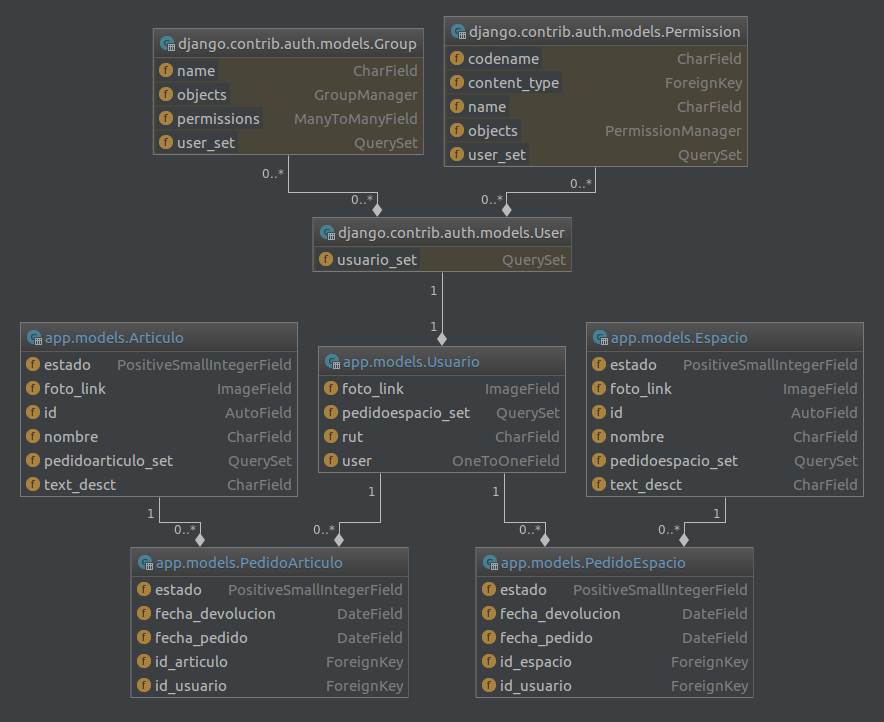
\includegraphics[width=0.5\textheight]{images/modelo_de_datos.png}
\caption{Diagrama del modelo de datos implementado} \label{LPUser}
\end{figure}
En este modelo se pueden distinguir tres niveles: un primer nivel generado automaticamente por Django en cuanto se utilizan sus modelos de Groups, Permission y User; un segundo nivel creado por el equipo donde se encuentran los elementos directamente relacionados con los requisitos que son los Artículos, Usuarios y Espacios; el último nivel es creado también por el equipo, pero son tablas relacionales entre los usuarios y artículos y espacios que representan los pedidos realizados por los usuarios y los resultados históricos de estas solicitudes.
Los modelos del primer nivel permiten generar un sistema de creación de usuario y logín con facilidad. Estos modelos disponen de nombre, apellido, correo, clave, permisos y grupos, todo ello por defecto dentro de Django. Así, podemos diferenciar una Persona Natural de un Administrador utilizando grupos, dando permisos por separado a cada grupo según lo indicado en los requisitos, así como poder guardar la información requerida por los usuarios. \\
Sin embargo, se hace necesario complementar esta información con datos adicionales que no corresponden al modelo de Django. Para ello, en el segundo nivel del modelo se extiende el usuario por defecto de Django con un usuario personalizado con nueva información adicional, como el rut y la foto de perfil; esta información servira para poblar de contenido el perfil del usuario. Además, consideramos tablas adicionales para los artículos y los espacios que dispondra el sistema para prestar a sus usuarios. La información que ahí se almacena servira para poder poblar las fichas de los artículos y espacios. \\
El último nivel, que posee las tablas relacionales entre usuario y artículo, y usuario y espacio; estas tablas almacenan la información de los pedidos hechos por un usuario, la fecha de pedido y devolución. Esta información se puede usar por el perfil del usuario como un registro histórico de sus pedidos, además de poder indicar al sistema que elementos se encuentran disponibles para que otros usuarios puedan pedir o no un artículo (según las fechas de los pedidos), así como informar a los administradores sobre la vigencia o caducidad de una solicitud (entre otros posibles). 

\newpage
\section{Cumplimiento Requisitos}
Los requisitos se dividieron en grupos a modo de facilitar el trabajo sobre cada uno de ellos, de forma tal que la funcionalidad base pudiera dar cuenta de un conjunto de ellos en lugar de tan solo uno. Por ejemplo, si el sistema requiere de la inscripción de un usuario, era necesario que el usuario pudiera crear su cuenta, pudiera inscribirse y pudiera salir de su cuenta.
De esta forma, los requisitos se dividieron en: Requisitos generales (1-2, 4-5, 7-8, 12, 14-15), landing page para personas naturales (16-18), perfil de usuario (23, 25-26, 28), ficha de artículo (37-40), landing page para administradores (51, 54-56).
Del primer grupo de requisitos, podemos ver como estos se cumplen en...
\texttt{
Requisitos generales:
	
	1. El sistema debe permitir que personas naturales creen cuentas en el sistema, solicitando su nombre, RUT, correo electrónico y una contraseña.
		[Página para registrarse donde los datos se guardan en BD]

	2. Todo usuario debe autentificarse para acceder al sistema, usando el correo electrónico que tiene registrado en el sistema y su contraseña.
		[Página para logearse.]

	4. El sistema debe considerar 2 tipos de usuarios: administrador y persona natural (estudiante, funcionario, etc.).
		[]

	5. El sistema debe permitir que personas naturales realicen reservas de artículos.
		[Página para reservar]

	7. El sistema debe llevar un historial de las reservas realizadas por una persona natural, registrándose el usuario, fecha y hora de la reserva.
		[Página del historial]

	8. El sistema debe llevar un historial de los préstamos autorizados por un
	administrador, registrándose el usuario, fecha y hora del préstamo.
		[POST/GET de la DB de cierta info.]

	12.La reserva de cualquier artículo debe realizarse al menos 1 hora antes de la fecha/hora de inicio del préstamo.
		[Quizás desabilitar el préstamo para cosas la siguente hora actual del servidor.]

	14.Solo se puede reservar artículos y espacios en días hábiles, en el horario 09:00 - 18:00.
		[if hora<18 and hora>9 bla...]
	
	15.Cada artículo y espacio debe tener un identificador único en el sistema.
		[ITEM:ID en la DB]
}
De los requisitos asociados al landing page para personas naturales, podemos ver como estos se cumplen en...
\texttt{
Landing page para personas naturales:
	
	16.El sistema debe permitir buscar artículos.
		[Página de búsqueda]
	
	17.El sistema solo se debe mostrar los artículos que cumplen con los criterios de búsqueda especificados por el usuario. Inicialmente, deben considerar los siguientes criterios: identificador, nombre del artículo, rango de fechas y estado (disponible, en préstamo, en reparación, perdido).
		[Gracias por decirme qué cosas deben estar en la base de datos :)]

	18.El sistema debe mostrar una grilla con los horarios en que están reservadas los espacios administrados por el CEI.
		[La grilla]	
}
Respecto del perfil de usuario, los requisitos que aquí se cumplen son...
\texttt{
Perfil del usuario (vista por el dueño del perfil):

	23.El sistema debe mostrar el nombre, RUT y correo electrónico del usuario.
		[Bienvenido: <USER> (<RUT>) <USERBLALBA>@<dominio>]
	
	25.El sistema debe mostrar si el usuario está habilitado para crear reservas y concretar préstamos.
		[USER_STATE==YES]
	
	26.El sistema debe mostrar un listado de las últimas 10 reservas realizadas por el usuario, ordenados por fecha (más nuevos al inicio de la lista), indicando cuales están pendientes, cuales fueron rechazadas y cuales ya fueron concretadas.
		[Historial junto con reservas acutales]

	28.El sistema deber permitir que el usuario marque una o más reservas pendientes y eliminarlas.
		[El Historial debe ser interactivo]	
}
Por otra parte, de los requisitos asociados a la ficha del artículo...
\texttt{
Ficha de un artículo:
	37.El sistema debe mostrar la siguiente información para un artículo: nombre, foto, texto descriptivo y estado actual (disponible, en préstamo, en reparación, perdido).
		[Modelo para los artículos]

	38.El sistema también debe mostrar un resumen de las fechas en las cuales ha sido reservado el artículo.
		[Historial por artículo]
	
	39.En el caso de los administradores, el sistema debe permitir gestionar la información de un artículo.
		[Herramientas de gestión para admins]

	40.En el caso de una persona natural, el sistema debe permitirle al usuario indicar que quiere reservar el artículo, indicando el rango de fecha y horas del préstamo solicitado.
		[Herraminetas de gestión para users]	
}
Finalmente, los requisitos asociados directamente con la landing page de los administradores...
\texttt{
Landing page administradores
	51.El sistema debe mostrar una grilla con los horarios en que están reservadas los espacios administrados por el CEI.
		[La grilla de las cosas.]

	54.El sistema debe mostrar un listado de todas las reservas pendientes en el sistema, ordenados por fecha (más nuevos al inicio de la lista).
			
	55.El sistema debe permitir que el administrador marque una o más reservas pendientes, pudiendo cambiar su estado a entregado o rechazado.
		
	56.El sistema debe mostrar un listado de todas los préstamos en el sistema, ordenados por fecha (más nuevos al inicio de la lista). El sistema debe permitir filtrar los préstamos por estado (vigentes, caducados, perdidos).}	
}
Cabe hacer notar que la funcionalidad desarrollada para una parte, se aprovecha también para otra parte del sistema.

\newpage
\section{Conclusiones}
Luego de haber realizado la implementación de las interfaces del sistema estudiado durante el curso, se pueden llegar a una serie de conclusiones, en base al trabajo realizado, las herramientas utilizadas y las metodologías aplicadas.\\
En cuanto al trabajo realizado, podemos ver como la organización por requisitos ayuda a organizar los objetivos y la funcionalidad deseada para una aplicación, eliminando las distracciones y las ideas que pueden surgir a medida que se implementan otras funcionalidades. De esta forma, el trabajo se hace más organizado, más directo y más sencillo para todos los que participan. Por otro lado, muchas veces los requisitos implican otras funcionalidades, lo cual complica los límites y las responsabilidades de los trabajadores: por ejemplo, si una persona se encuentra encargada de desarrollar modelos, y otra se encuentra encargada de desarrollar un sistema de login, ambas partes se relacionan con los permisos de usuarios y la posibilidad de hacer préstamos. ¿Quién es el responsable de que el usuario pueda, efectivamente, hacer el pedido? \\
Las herramientas utilizadas, en particular Git, ayudan a superar estos problemas y ha hacer que el trabajo sea más armonioso. Si una parte no está resuelta o si falta funcionalidad, los responsables de las partes individuales pueden compartir sus inquietudes y resolver aquello que impide que su código funcione. De la misma forma, Django ayuda a separar las responsabilidades, asegurando que gran parte del sistema pueda funcionar de forma autonoma a las otras (es decir, desarrollar un frontend independiente del desarrollo del backend, pero que asume que el otro estará funcionando para poder tener en "andando" el sistema). \\
Finalmente, la metodología de trabajo tipo Scrum que se utilizó ayuda a acelerar los resultados deseados del trabajo. Poder separar el trabajo no solo en fronend y backend, si no que en "features", aseguraba el avance constante del quehacer de cada uno de los miembros del trabajo.


% FIN DEL DOCUMENTO
\end{document}
